\section{About Kalman and The Filter}

\subsection{On Rudolf E. Kalman}
\begin{frame}
   \frametitle{On Rudolf E. Kalman}

		\begin{itemize}
			\item Born in Budapest, Hungary, May 19, 1930
			\item Passed away in Gainsville, Florida, July 2, 2016
			\item Emigrated to USA in 1943
			\item Bachelor and Master in EE at MIT, 1953 and 1954, respectively
			\item Ph.D. at Columbia University, 1957 (Advisor: J. R. Ragazzini)
			\item Institutions: Stanford University, University of Floria, ETC Zurich (and more)
		\end{itemize}
		
		\begin{figure}
		\centering
			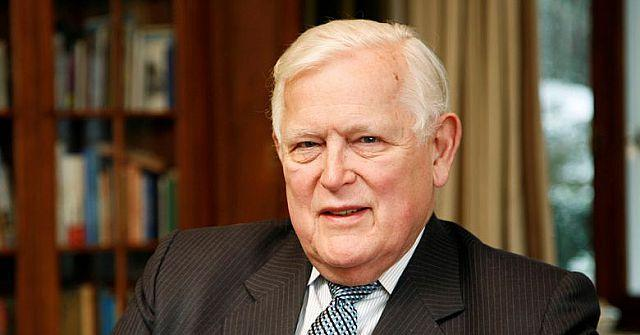
\includegraphics[width=0.70\textwidth]{Figures/Background/R. E. Kalman.jpg}
		\label{fig:REKalman}
		\caption{Rudolf E. Kalman}
	\end{figure}
	This is where it all started: \cite{Henrik_KF}	
\end{frame}
%-----------------------------------------------------

\subsection{The Filter}
\begin{frame}
   \frametitle{The Filter}
		\begin{itemize}
			\item The filter invented by R. E. Kalman in the 1960s, based on the seminal papers:
			    \begin{enumerate}
			        \item R. E. Kalman: Contribution to the Theory of Optimal Control (1960)
			        \item \textbf{R. E. Kalman: A New Approach to Linear Filtering and Prediction Problems (1960)}
			        \item R. E. Kalman: Mathematical Description of Linear Dynamical Systems (1963)
			    \end{enumerate}
			\item (2) describes a recursive solution to the discrete-data linear filtering problem---Kalman Filter
			
			\item Enormous impact on the fields of \textbf{linear systems theory, statistics, signal processing, identification, feedback control, and adaptive systems}
			
			\item Additionally, on motivating new formulations of feasible filtering problems outside the linear domain. 
			
			\item Kalman Filtering is used extensively, mainly for \textit{target tracking}. However, it can be applied to any field where \textit{estimation and prediction} are required, e.g., location and navigation systems, control systems, computer graphics, and much more.
		\end{itemize}
		
		\vspace{10pt}
		\textbf{Estimation problem}: Estimating hidden (unknown) states based on a series of measurements.
		
		\begin{itemize}
		    \item For example, a GPS receiver provides location and velocity estimation, where location and velocity are the hidden states and differential time of the satellites' signals' arrival are the measurements.
		    \item Challenge is providing an accurate and precise estimation of the hidden states in the \textbf{presence of uncertainty}.
		    \begin{itemize}
		        \item In GPS receivers, the measurement uncertainty depends on many external factors such as thermal noise, atmospheric effects, slight changes in satellite positions, receiver clock precision, etc.
		    \end{itemize}
		   \item The Kalman Filter produces estimates of hidden variables based on inaccurate and uncertain measurements.  
		\end{itemize}
		
		
\end{frame}
%-----------------------------------------------------
\begin{frame}
   \frametitle{Filtering}
   
   Estimate the current value of the stochastic signal, using the history and current value of another observed stochastic process; e.g., using the measurements $Y_k = \{y_i, i\leq k\}$, we want to estimate $\hat{x}_{k + m}$. It leads to three cases:
   	\begin{figure}
		\centering
			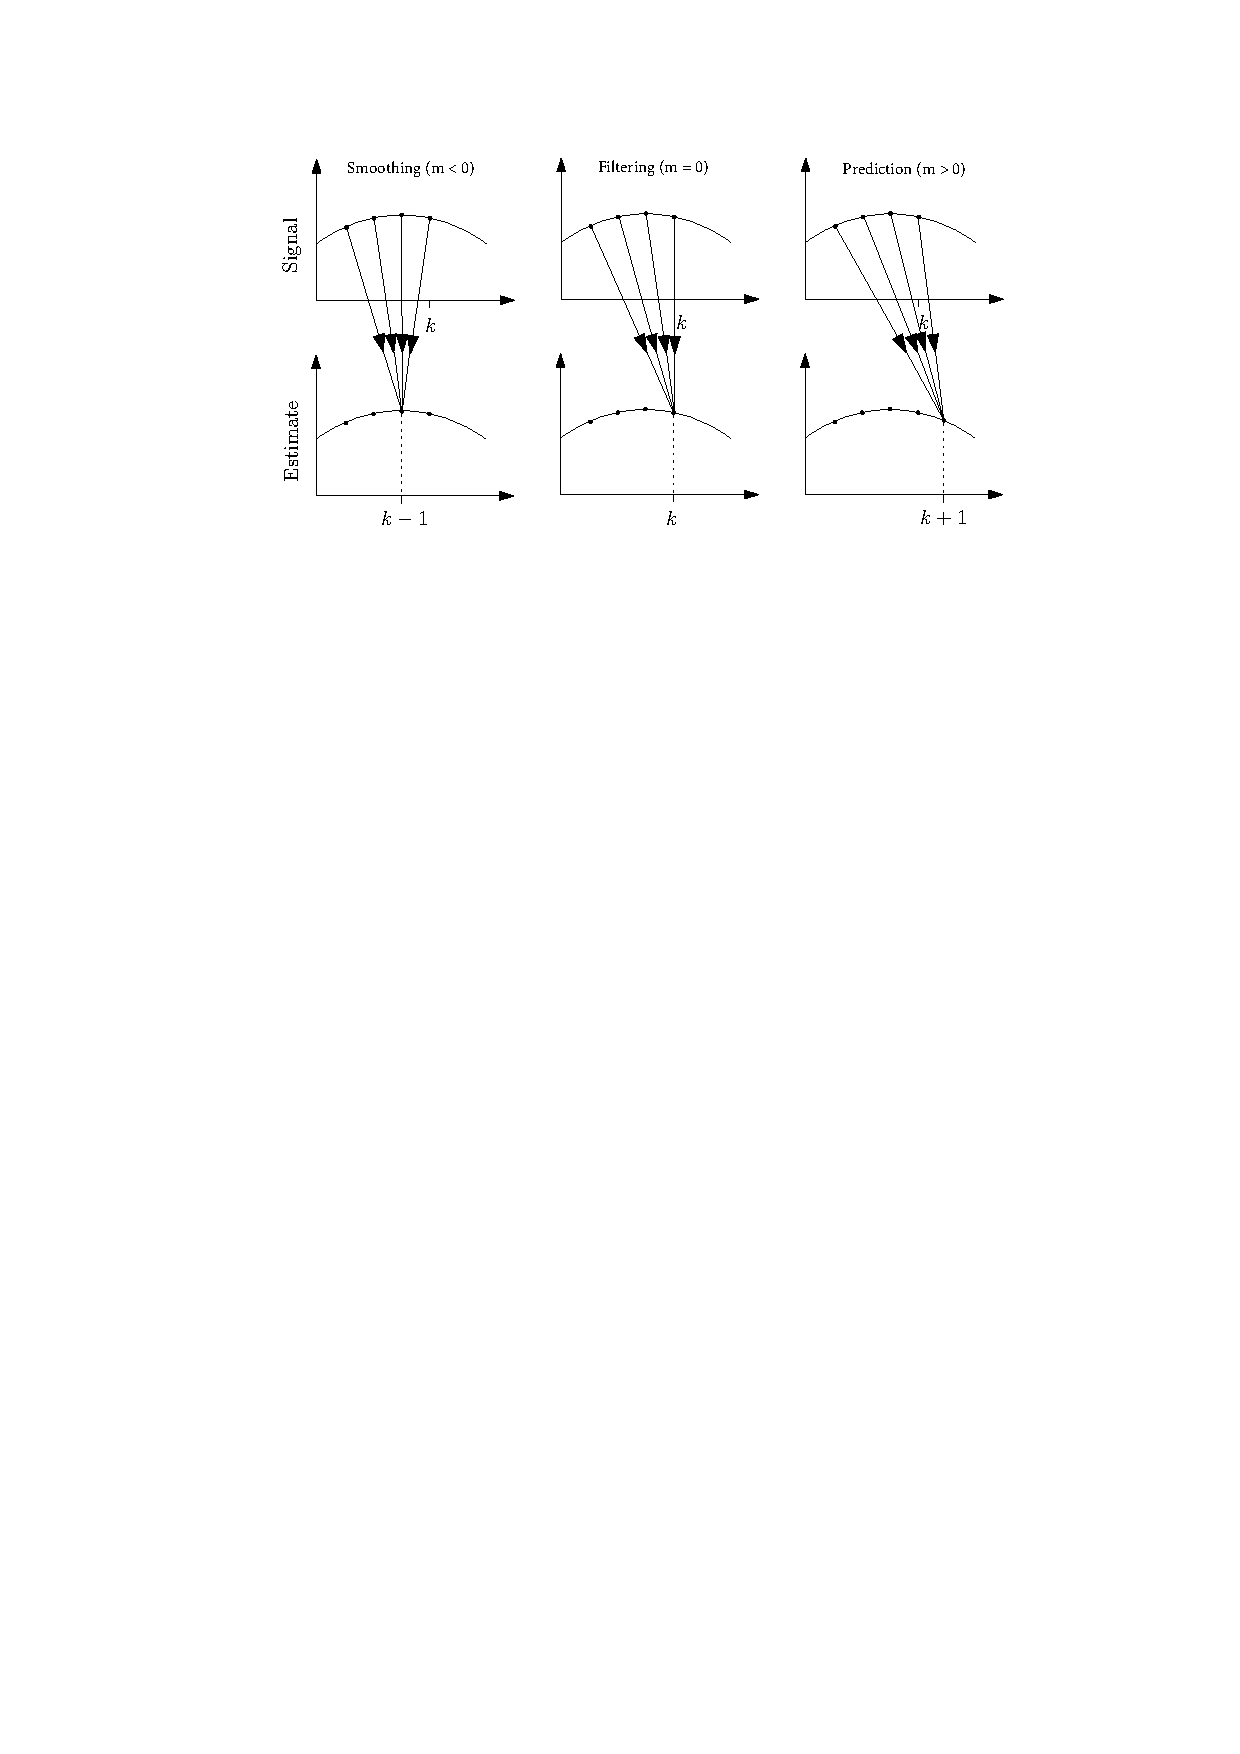
\includegraphics[width=0.70\textwidth]{Figures/Background/Smoothing, Filtering, and Prediction.pdf}
		\label{fig:WirelessVision}
		\caption{Smoothing, filtering, prediction}
	\end{figure}
	\begin{itemize}
	    \item \textbf{Smoothing}: Estimation of the past state-variable at the present time
	    \item \textbf{Filtering}: Estimating the present state-variable at the present time
	    \item \textbf{Prediction}: Estimating the future state-variable at the present time
	\end{itemize}

\end{frame}


\begin{frame}\frametitle{The Necessity of Prediction}
   
   \textbf{Radar tracking algorithm}
    
    \begin{columns}\column{0.5\textwidth}
        
    \begin{itemize}
        \item The tracking radar sends a pencil beam in the direction of the target.
        \item In every track cycle of $\Delta t$, the radar revisits the target by sending a dedicated track beam in the direction of the target.    
        \item After sending the beam, the radar estimates the current target position and velocity. The radar also estimates (or predicts) the target position at the next track beam.
    \end{itemize}
    \begin{figure}
		\centering
			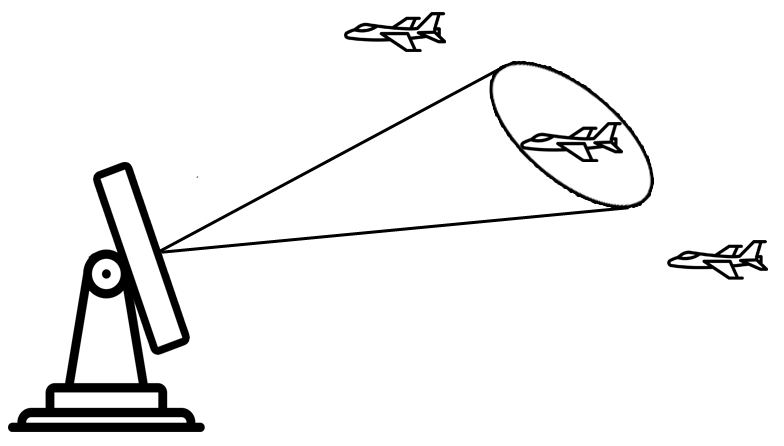
\includegraphics[width=0.8\textwidth]{Figures/Background/tracking_radar.png}
		\label{fig:Radar_Tracking}
	\end{figure} 
        
    \column{0.5\textwidth}
    \vspace{-15pt}
    \begin{itemize}
        \item The future target position can be easily calculated using Newton's motion equations:
        \vspace{-8pt}
        $$x = x_0 + v_0 \Delta t + \frac{1}{2}a\Delta t^2$$
        where\\ 
        $x$~~~is the target's position\\
        $x_0$~~is the target's initial position\\
        $v_0$~~is the target's initial velocity\\
        $a$~~~is the target's acceleration\\
        $\Delta t$ is the track cycle\\
    \end{itemize}
    
    In 3D, it can be written as a system of equations
    \begin{align*}
     x = & x_0 + v_{x0} \Delta t + \frac{1}{2}a_x\Delta t^2\\\nonumber
     y = & y_0 + v_{y0} \Delta t + \frac{1}{2}a_y\Delta t^2\\\nonumber
     z = & z_0 + v_{z0} \Delta t + \frac{1}{2}a_z\Delta t^2\\\nonumber
    \end{align*}
    \end{columns}
   The above set of equations is called a \textbf{Dynamic Model} (or a \textbf{State Space Model}). The Dynamic Model describes the relationship between input and output.
\end{frame}

%-----------------------------------------------------
\begin{frame}{Constant Acceleration}
    \begin{figure}
		\centering
			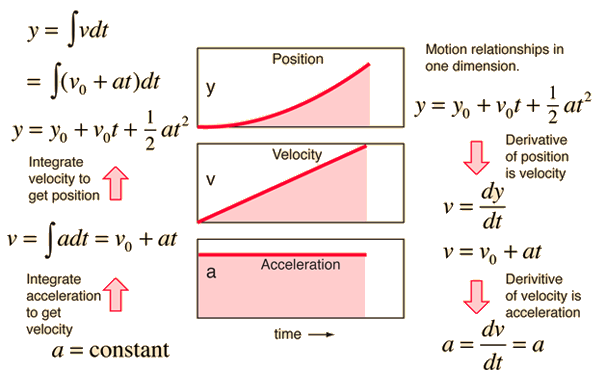
\includegraphics[width=0.7\textwidth]{Figures/Background/Constant Acceleration.png}
		\label{fig:Radar_Tracking}
	\end{figure}     
    
\end{frame}

%-----------------------------------------------------
\begin{frame}{Terminologies using tracking example}
    
    
    \begin{itemize}
    
        \item \textbf{Dynamic or State Space Model:} Describes the relationship between input and output. 
        \item \textbf{System State}
    
            \begin{itemize}
                \item The target parameters $[x, y, z, v_x, v_y, v_z, a_x, a_y, a_z]$ are called a \textbf{System State}. 
                
                \item The current state is the input to the prediction algorithm and the next state (the target parameters at the next time interval) is the algorithm's output.
            \end{itemize}
    
        \item So, if the current state and the dynamic model are known, the next target state can be easily predicted? \textbf{Well, not really!}
        
        \item \textbf{Measurement Noise:} The radar measurement is not absolute; it includes a random error (or uncertainty). The error magnitude depends on many parameters, such as radar calibration, the beam width, and the signal-to-noise ratio of the returned echo. \textit{The error included in the measurement is called Measurement Noise.}
        
        
        \item \textbf{Process Noise:} The target motion is not strictly aligned to motion equations due to external factors such as wind, air turbulence, and pilot maneuvers. \textit{The dynamic model error (or uncertainty) is called Process Noise.}
    \end{itemize}
    
    \begin{framed}
    Due to Measurement Noise and Process Noise, the estimated target position can be far away from the actual target position. In this case, the radar might send the track beam in the wrong direction and miss the target.
    \end{framed}
    
\end{frame}

%-----------------------------------------------------


